%\section{Data and Calibration Results}
This appendix presents European call option and stock data used as well as the estimated marginal parameters from the calibration procedure presented in Appendix \ref{appendix: Calibration Procedure}. 

\section{Data}
\label{appendix: Data}
The data used for calibration are obtained from the LSEG Workspace terminal. As such, the data set is assumed to be clean, and no additional data preprocessing is performed. Stock price data are collected over the period from 2024‑05‑14 to 2026‑05‑13 at a daily frequency at market close, resulting in a total of 498 observations per stock. Option prices are collected on 2026‑05‑13 at market close, with times to maturity of at most one year. An overview of the collected data is provided in Tables \ref{tab: stock data} and \ref{tab: option-sample-overviews}, while the data itself can be found in \cite{mycode}.

\begingroup
\scriptsize
\renewcommand{\arraystretch}{0.98}
\setlength{\tabcolsep}{2pt}
\setlength{\LTleft}{0pt}
\setlength{\LTright}{0pt}
\setlength{\LTcapwidth}{\linewidth}

\newcommand{\optionsampleblock}[9]{%
    \begin{minipage}[t]{\linewidth}
        \vspace{0pt}
        \begin{tabular*}{\linewidth}{@{\extracolsep{\fill}}lrr@{}}
            \toprule
            \multicolumn{3}{c}{\textbf{#1}} \\
            \midrule
            Valuation date & \multicolumn{2}{r}{#2} \\
            Spot price (CHF) & \multicolumn{2}{r}{#3} \\
            Total samples & \multicolumn{2}{r}{#4} \\
            \addlinespace[0.25em]
            \midrule
            Expiry date & \shortstack[r]{Days to\\maturity} & Samples \\
            \midrule
            #5 \\
            #6 \\
            #7 \\
            #8 \\
            #9 \\
            \bottomrule
        \end{tabular*}
    \end{minipage}%
}

\begin{longtable}{@{}p{\dimexpr\linewidth/2-0.5em\relax}@{\hspace{1em}}p{\dimexpr\linewidth/2-0.5em\relax}@{}}

    \endfirsthead

    \endhead

    \midrule
    \multicolumn{2}{r}{\emph{Continued on next page}} \\
    \endfoot

    \bottomrule
    \\[0.05em]
    \caption{Option sample overviews for all underlyings. Prices are quoted in the Swiss Franc (CHF).
    \label{tab: option-sample-overviews}}\\
    \endlastfoot

    \optionsampleblock{ABBN}{2026-05-14}{82.86}{228}
        {2026-06-19 & 36 & 62}
        {2026-07-17 & 64 & 37}
        {2026-09-18 & 127 & 43}
        {2026-12-18 & 218 & 54}
        {2027-03-19 & 309 & 32}
    &
    \optionsampleblock{ALCC}{2026-05-14}{49.61}{111}
        {2026-06-19 & 36 & 32}
        {2026-07-17 & 64 & 32}
        {2026-09-18 & 127 & 15}
        {2026-12-18 & 218 & 18}
        {2027-03-19 & 309 & 14}
    \\[1.0em]

    \optionsampleblock{CFR}{2026-05-14}{156.55}{269}
        {2026-06-19 & 36 & 59}
        {2026-07-17 & 64 & 34}
        {2026-09-18 & 127 & 70}
        {2026-12-18 & 218 & 76}
        {2027-03-19 & 309 & 30}
    &
    \optionsampleblock{GALD}{2026-05-14}{158.35}{119}
        {2026-06-19 & 36 & 36}
        {2026-07-17 & 64 & 29}
        {2026-09-18 & 127 & 17}
        {2026-12-18 & 218 & 25}
        {2027-03-19 & 309 & 12}
    \\[1.0em]

    \optionsampleblock{GEBN}{2026-05-14}{503.40}{120}
        {2026-06-19 & 36 & 36}
        {2026-07-17 & 64 & 30}
        {2026-09-18 & 127 & 17}
        {2026-12-18 & 218 & 21}
        {2027-03-19 & 309 & 16}
    &
    \optionsampleblock{GIVN}{2026-05-14}{2683.00}{182}
        {2026-06-19 & 36 & 53}
        {2026-07-17 & 64 & 31}
        {2026-09-18 & 127 & 34}
        {2026-12-18 & 218 & 35}
        {2027-03-19 & 309 & 29}
    \\[1.0em]

    \optionsampleblock{HOLN}{2026-05-14}{76.26}{177}
        {2026-06-19 & 36 & 50}
        {2026-07-17 & 64 & 31}
        {2026-09-18 & 127 & 32}
        {2026-12-18 & 218 & 34}
        {2027-03-19 & 309 & 30}
    &
    \optionsampleblock{LONN}{2026-05-14}{474.20}{177}
        {2026-06-19 & 36 & 48}
        {2026-07-17 & 64 & 34}
        {2026-09-18 & 127 & 31}
        {2026-12-18 & 218 & 35}
        {2027-03-19 & 309 & 29}
    \\[1.0em]

    \optionsampleblock{NESN}{2026-05-14}{76.88}{188}
        {2026-06-19 & 36 & 49}
        {2026-07-17 & 64 & 33}
        {2026-09-18 & 127 & 35}
        {2026-12-18 & 218 & 42}
        {2027-03-19 & 309 & 29}
    &
    \optionsampleblock{NOVN}{2026-05-14}{116.80}{182}
        {2026-06-19 & 36 & 44}
        {2026-07-17 & 64 & 29}
        {2026-09-18 & 127 & 37}
        {2026-12-18 & 218 & 44}
        {2027-03-19 & 309 & 28}
    \\[1.0em]

    \optionsampleblock{PGHN}{2026-05-14}{883.60}{173}
        {2026-06-19 & 36 & 47}
        {2026-07-17 & 64 & 28}
        {2026-09-18 & 127 & 30}
        {2026-12-18 & 218 & 41}
        {2027-03-19 & 309 & 27}
    &
    \optionsampleblock{ROPC}{2026-05-14}{320.00}{205}
        {2026-06-19 & 36 & 48}
        {2026-07-17 & 64 & 29}
        {2026-09-18 & 127 & 48}
        {2026-12-18 & 218 & 53}
        {2027-03-19 & 309 & 28}
    \\[1.0em]

    \optionsampleblock{SDZ}{2026-05-14}{67.76}{151}
        {2026-06-19 & 36 & 35}
        {2026-07-17 & 64 & 26}
        {2026-09-18 & 127 & 32}
        {2026-12-18 & 218 & 33}
        {2027-03-19 & 309 & 25}
    &
    \optionsampleblock{SGSN}{2026-05-14}{84.68}{153}
        {2026-06-19 & 36 & 38}
        {2026-07-17 & 64 & 29}
        {2026-09-18 & 127 & 29}
        {2026-12-18 & 218 & 29}
        {2027-03-19 & 309 & 28}
    \\[1.0em]

    \optionsampleblock{SIKA}{2026-05-14}{140.95}{127}
        {2026-06-19 & 36 & 36}
        {2026-07-17 & 64 & 20}
        {2026-09-18 & 127 & 23}
        {2026-12-18 & 218 & 28}
        {2027-03-19 & 309 & 20}
    &
    \optionsampleblock{SLHN}{2026-05-14}{837.60}{201}
        {2026-06-19 & 36 & 52}
        {2026-07-17 & 64 & 36}
        {2026-09-18 & 127 & 40}
        {2026-12-18 & 218 & 43}
        {2027-03-19 & 309 & 30}
    \\[1.0em]

    \optionsampleblock{SCMN}{2026-05-14}{678.00}{175}
        {2026-06-19 & 36 & 48}
        {2026-07-17 & 64 & 29}
        {2026-09-18 & 127 & 32}
        {2026-12-18 & 218 & 37}
        {2027-03-19 & 309 & 29}
    &
    \optionsampleblock{SRENH}{2026-05-14}{119.45}{174}
        {2026-06-19 & 36 & 51}
        {2026-07-17 & 64 & 34}
        {2026-09-18 & 127 & 29}
        {2026-12-18 & 218 & 32}
        {2027-03-19 & 309 & 28}
    \\[1.0em]

    \optionsampleblock{UBSG}{2026-05-14}{36.22}{173}
        {2026-06-19 & 36 & 50}
        {2026-07-17 & 64 & 33}
        {2026-09-18 & 127 & 30}
        {2026-12-18 & 218 & 30}
        {2027-03-19 & 309 & 30}
    &
    \optionsampleblock{ZURN}{2026-05-14}{563.00}{218}
        {2026-06-19 & 36 & 52}
        {2026-07-17 & 64 & 30}
        {2026-09-18 & 127 & 62}
        {2026-12-18 & 218 & 46}
        {2027-03-19 & 309 & 28}
    \\

\end{longtable}

\endgroup

\begin{table}[h]
    \centering
    \begin{tabular}{lcrr}
        \toprule
        Asset & Ticker & Initial Price & Final Price \\
        \midrule
        ABB Ltd & ABBN & 46.88 & 82.86 \\
        Alcon AG & ALCC & 73.06 & 49.61 \\
        Compagnie Financière Richemont SA & CFR & 155.75 & 156.55 \\
        Galderma Group AG & GALD & 97.95 & 158.35 \\
        Geberit AG & GEBN & 597.20 & 503.40 \\
        Givaudan SA & GIVN & 3997.00 & 2683.00 \\
        Holcim AG & HOLN & 49.50 & 76.26 \\
        Lonza Group AG & LONN & 572.20 & 474.20 \\
        Nestlé SA & NESN & 85.21 & 76.88 \\
        Novartis AG & NOVN & 90.52 & 116.80 \\
        Partners Group Holding AG & PGHN & 1187.50 & 883.60 \\
        Roche Holding AG & ROPC & 259.30 & 320.00 \\
        Sandoz Group AG & SDZ & 38.15 & 67.76 \\
        SGS SA & SGSN & 85.70 & 84.68 \\
        Sika AG & SIKA & 217.80 & 140.95 \\
        Swiss Life Holding AG & SLHN & 826.20 & 837.60 \\
        Swisscom AG & SCMN & 538.00 & 678.00 \\
        Swiss Re AG & SRENH & 147.25 & 119.45 \\
        UBS Group AG & UBSG & 27.23 & 36.22 \\
        Zurich Insurance Group AG & ZURN & 573.00 & 563.00 \\
        \bottomrule
    \end{tabular}
    \caption{Summary of stock price data from 2024-05-14 through 2026-05-13. Prices are quoted in the Swiss Franc (CHF).}
    \label{tab: stock data}
\end{table}

\section{Calibration results}
\label{appendix: calibration results}
\subsection{Estimated parameters}
To estimate the parameters $\mu$, $\sigma$, $\theta$, and $\nu$, we use the calibration procedure proposed in Appendix \ref{appendix: Calibration Procedure}. The FFT parameters were $N_{\text{FFT}}=1024$, $\eta=0.25$, $\alpha=1.5$, which are the same parameters \textcite{carr1999option} use. When estimating the parameters using the DE algorithm, we asserted the bounds: $\sigma \in (0.05,0.6)$, $\theta \in (-2.0, -0.0001)$, and $\nu \in (0.001, 0.45)$ to keep the estimated parameters economically interpretable. When estimating $\mu$, we cap empirical log-returns to the 95-th quantile in order to make a more conservative estimation. The risk-free rate is the Swiss Average Rate Overnight (SARON) and is $\delta\approx 0\%$ per May 14th, 2026. The resulting estimations can be found in Table~\ref{tab: parameter estimates percent appendix}. The log-return correlation matrix can be found in Figure~\ref{fig: log-return corr matrix}.

\begin{table}[!htbp]
    \centering
    \begin{tabular}{lrrrr}
        \toprule
        TKR & $\mu$ (\%) & $\sigma$ (\%) & $\theta$ (\%) & $\nu$ (\%) \\
        \midrule
        ABB   &  12.71 & 29.42 & -36.63 &  8.31 \\
        ALCC  &  -8.35 & 27.31 & -28.01 &  8.87 \\
        CFR   &   0.03 & 30.20 &  -0.01 &  0.94 \\
        GALD  &  18.74 & 27.61 & -84.67 &  3.64 \\
        GEBN  &  -0.70 & 21.32 & -15.62 &  1.13 \\
        GIVN  &  -5.89 & 25.68 & -33.67 & 38.18 \\
        HOLN  &  13.36 & 25.21 & -29.84 &  4.99 \\
        LONN  &   1.13 & 27.89 & -28.42 &  5.73 \\
        NESN  &  -3.45 & 18.48 & -31.11 &  8.21 \\
        NOVN  &   6.16 & 20.60 & -25.11 &  1.83 \\
        PGHN  &  -6.21 & 23.76 & -79.28 &  1.19 \\
        ROPC  &   6.76 & 21.61 & -16.70 &  1.88 \\
        SDZ   &  18.30 & 28.44 & -62.67 &  3.45 \\
        SGSN  &   3.86 & 19.74 & -42.65 & 10.52 \\
        SIKA  & -12.97 & 30.29 & -22.27 &  9.68 \\
        SLHN  &   6.08 & 18.93 &  -0.01 &  0.66 \\
        SCMN  &   7.67 & 19.56 & -22.00 & 45.00 \\
        SRENH &   2.24 & 22.56 & -31.83 & 15.14 \\
        UBSG  &   8.61 & 25.65 & -44.70 &  5.18 \\
        ZURN  &   3.86 & 17.65 & -25.12 &  2.29 \\
        \bottomrule
    \end{tabular}
    \caption{Estimated model parameters.}
    \label{tab: parameter estimates percent appendix}
\end{table}

\begin{figure}[!htbp]
  \centering
  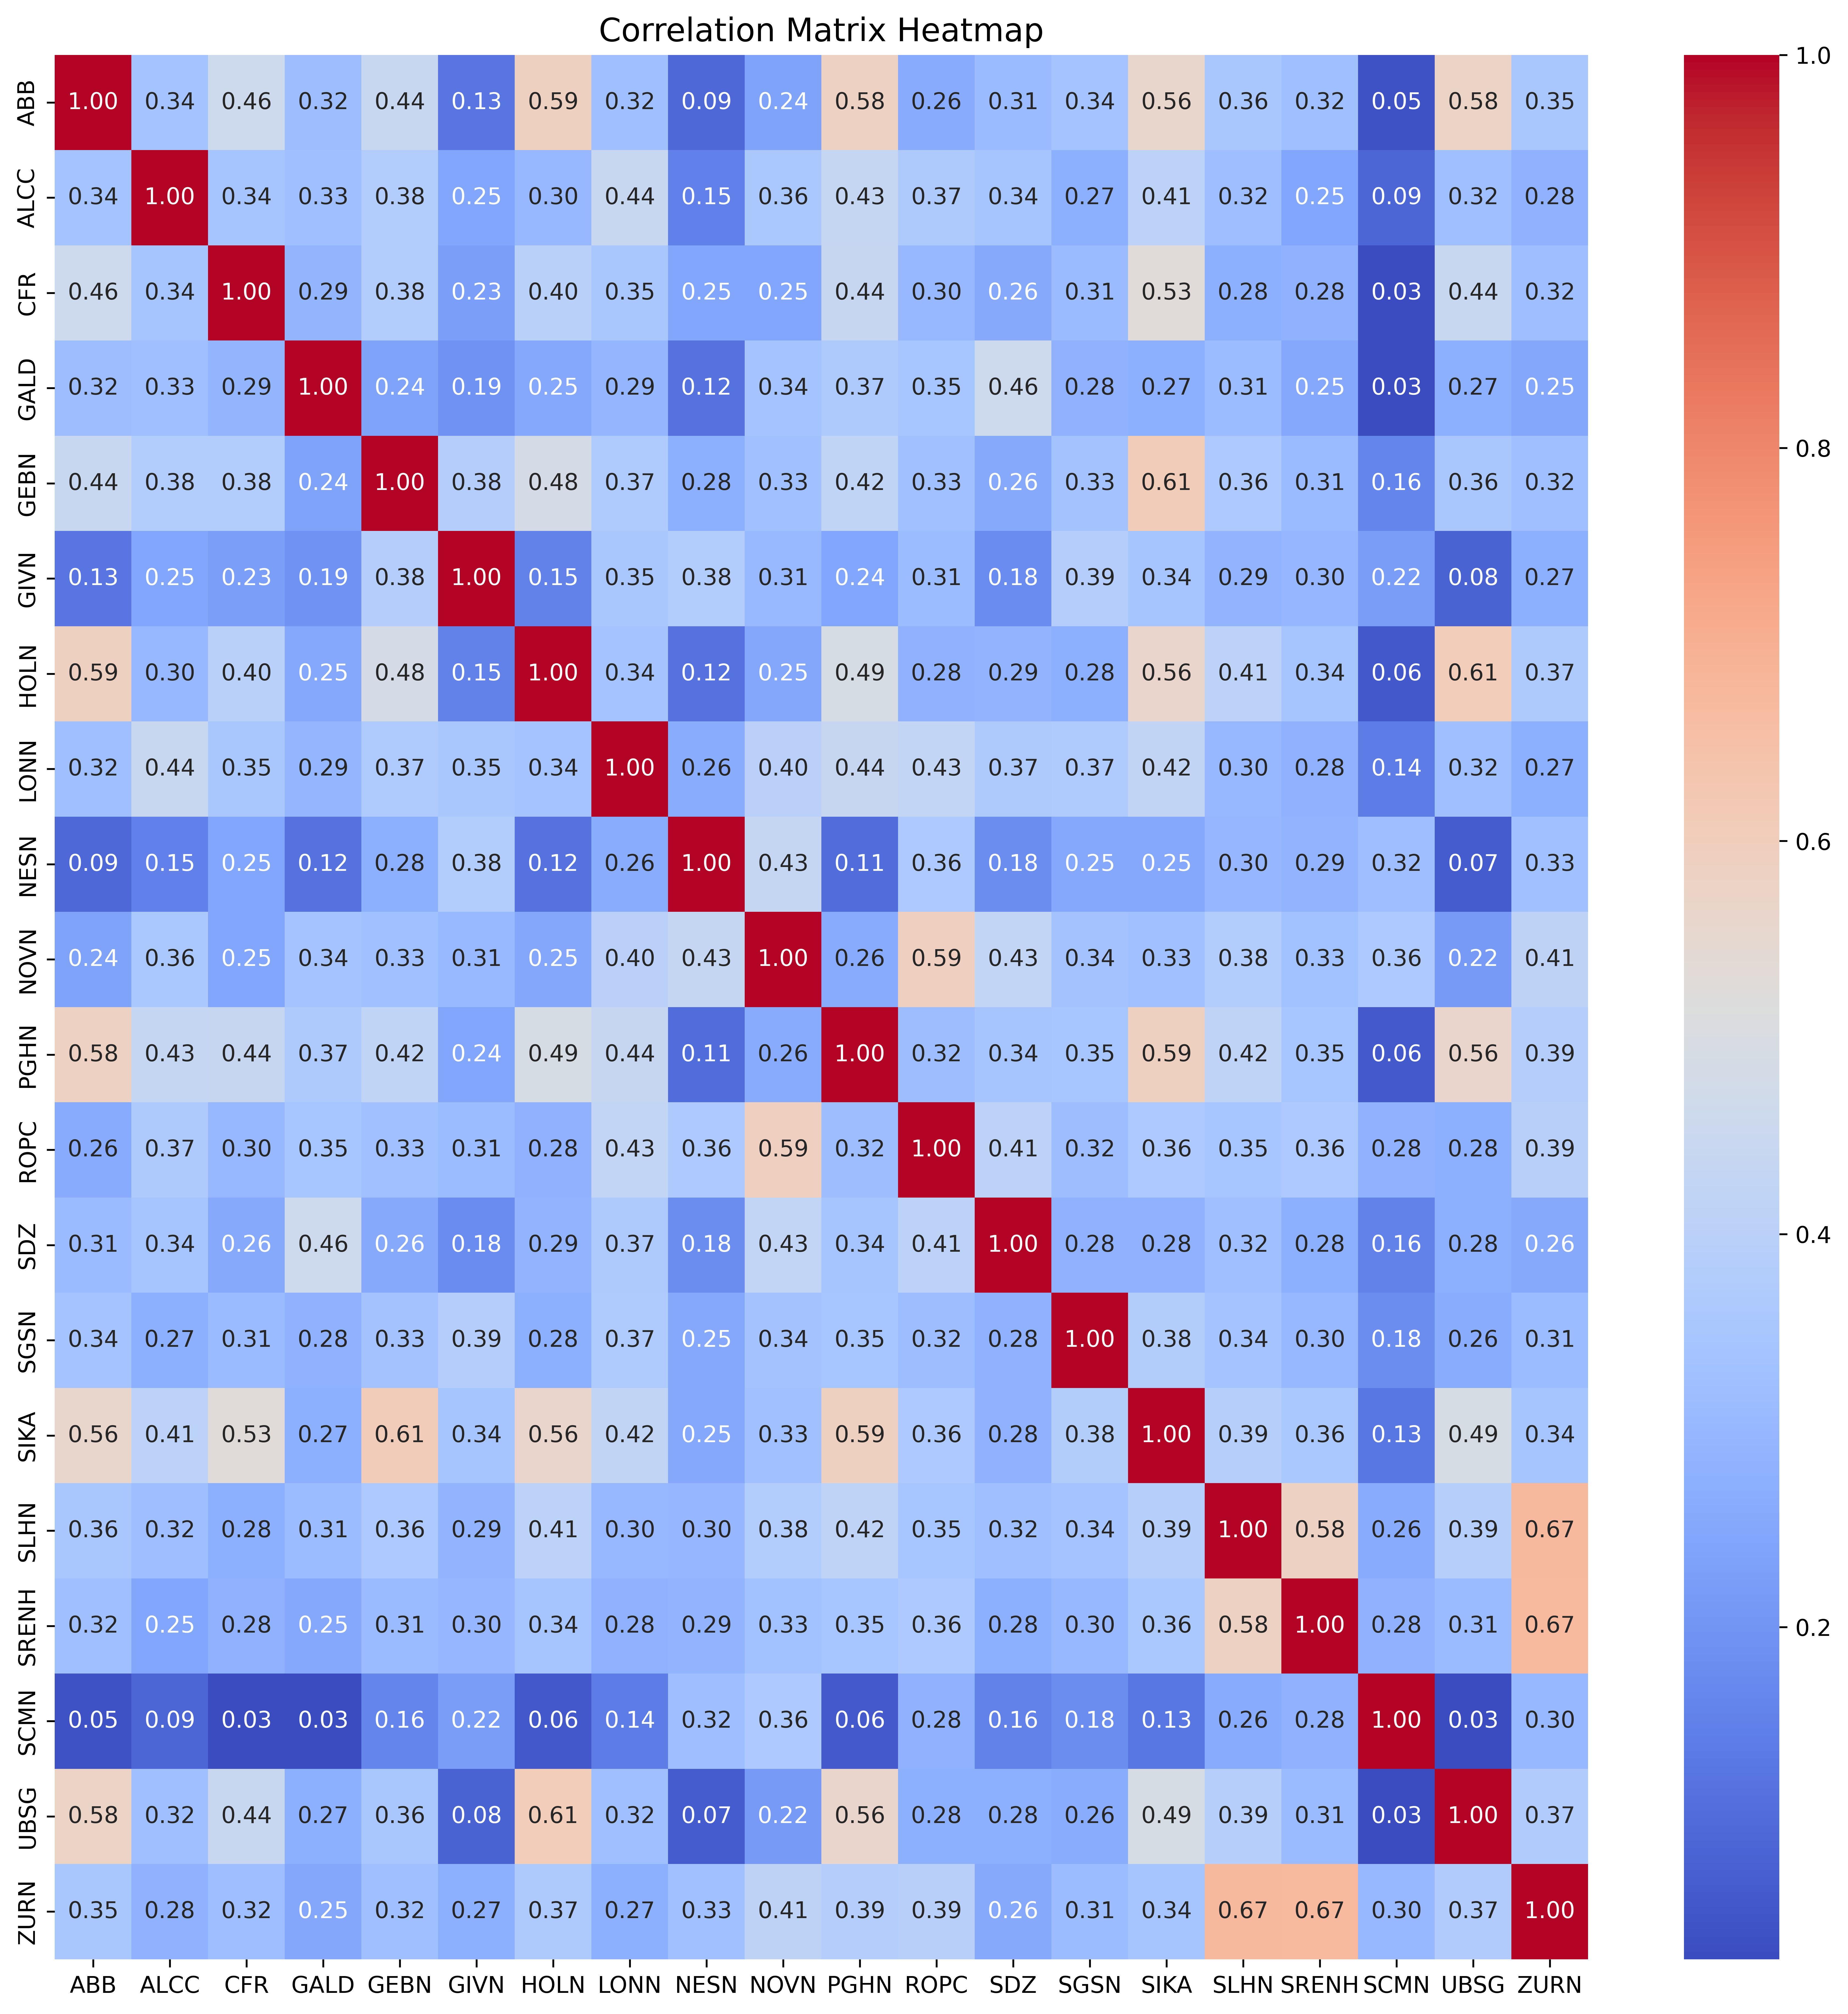
\includegraphics[width=\textwidth]{Plots/Calibration/log_return_corr_matrix.png}
  \caption{Log-return correlation matrix}
  \label{fig: log-return corr matrix}
\end{figure}

\subsection{Error metrics and plots}
The error metrics used to evaluate the estimated parameters across all strikes and maturities are the Mean Absolute Error (MAE), the Root Mean-Squared Error (RMSE), and the Mean Absolute Percentage Error (MAPE), given by \eqref{eqn: MAE}, \eqref{eqn: RMSE}, and \eqref{eqn: MAPE}, respectively. 
\begin{equation}
    \text{MAE} = \frac{1}{MN} \sum_{m=1}^M\sum_{n=1}^N \left| C_{T_m}^{\text{Model}}(s,K_n) - C_{m,n}^{\text{Market}} \right|
    \label{eqn: MAE}
\end{equation}
\begin{equation}
    \text{RMSE} = \sqrt{\frac{1}{MN} \sum_{m=1}^M\sum_{n=1}^N \left(C_{T_m}^{\text{Model}}(s,K_n) - C_{m,n}^{\text{Market}}\right)^2}
    \label{eqn: RMSE}
\end{equation}
\begin{equation}
    \text{MAPE} = \frac{100}{MN} \sum_{m=1}^M\sum_{n=1}^N \left| \frac{C_{T_m}^{\text{Model}}(s,K_n) - C_{m,n}^{\text{Market}}}{C_{m,n}^{\text{Market}}} \right|.
    \label{eqn: MAPE}
\end{equation}

The error metrics \eqref{eqn: MAE}--\eqref{eqn: MAPE} have different interpretations. MAE captures the average magnitude of pricing deviations without considering the direction of the deviation. It provides a measure for overall model accuracy. RMSE emphasizes larger errors, making it particularly sensitive to large mispricings. Finally, MAPE expresses errors relative to market prices, making it particularly useful for assessing whether low-priced instruments are priced accurately. 

Pricing errors for each underlying can be found in Table~\ref{tab: error-metric-overviews}. Note that pricing errors are relatively small across all underlying assets except Partners Group Holding (PGHN).

\begingroup
\scriptsize
\renewcommand{\arraystretch}{0.98}
\setlength{\tabcolsep}{3pt}

\newcommand{\errormetricblock}[4]{%
    \begin{minipage}[t]{\linewidth}
        \vspace{0pt}
        \begin{tabular*}{\linewidth}{@{\extracolsep{\fill}}lr@{}}
            \toprule
            \multicolumn{2}{c}{\textbf{#1}} \\
            \midrule
            Metric & Value \\
            \midrule
            MAE & $#2$ \\
            RMSE & $#3$ \\
            MAPE (\%) & $#4$ \\
            \bottomrule
        \end{tabular*}
    \end{minipage}%
}

\begin{longtable}{@{}p{0.485\textwidth}@{\hspace{0.03\textwidth}}p{0.485\textwidth}@{}}

    \endfirsthead

    \endhead

    \midrule
    \multicolumn{2}{r}{\emph{Continued on next page}} \\
    \endfoot

    \bottomrule
    \\[0.2em]
    \caption{Error metrics for all underlyings.\label{tab:error-metric-overviews}}
    \label{tab:  error-metric-overviews}\\
    \endlastfoot

    \errormetricblock{ABBN}{0.116918}{0.161007}{3.747744}
    &
    \errormetricblock{ALCC}{0.065518}{0.092814}{8.608676}
    \\[1.0em]

    \errormetricblock{CFR}{0.686083}{0.908786}{7.469491}
    &
    \errormetricblock{GALD}{0.265190}{0.356102}{4.030166}
    \\[1.0em]

    \errormetricblock{GEBN}{1.010899}{1.690254}{6.993848}
    &
    \errormetricblock{GIVN}{7.633179}{13.332721}{15.814692}
    \\[1.0em]

    \errormetricblock{HOLN}{0.860288}{1.024028}{11.666620}
    &
    \errormetricblock{LONN}{0.538848}{0.869958}{12.044501}
    \\[1.0em]

    \errormetricblock{NESN}{0.100446}{0.131476}{7.265444}
    &
    \errormetricblock{NOVN}{0.336908}{0.699478}{3.111208}
    \\[1.0em]

    \errormetricblock{PGHN}{17.017618}{22.402186}{22.797090}
    &
    \errormetricblock{ROPC}{0.874842}{1.675453}{3.485799}
    \\[1.0em]

    \errormetricblock{SDZ}{0.106628}{0.143644}{4.105436}
    &
    \errormetricblock{SGSN}{0.116536}{0.152647}{5.263105}
    \\[1.0em]

    \errormetricblock{SIKA}{0.175852}{0.280050}{9.908205}
    &
    \errormetricblock{SLHN}{2.232442}{3.297510}{8.818372}
    \\[1.0em]

    \errormetricblock{SCMN}{1.142384}{2.044142}{11.760861}
    &
    \errormetricblock{SRENH}{0.149317}{0.223762}{11.477619}
    \\[1.0em]

    \errormetricblock{UBSG}{0.081952}{0.117784}{2.462055}
    &
    \errormetricblock{ZURN}{1.287465}{1.791158}{6.312769}
    \\

\end{longtable}
\endgroup